% 页面设置
\documentclass[12pt, a4paper]{article} % 字号:12,纸张:A4
\usepackage[top=2.54cm, bottom=2.54cm, left=3.18cm,right=3.18cm]{geometry} % 页边距设置
% 字体设置
\usepackage[UTF8]{ctex}
\usepackage{fontspec} % 设置字体
%\setCJKmainfont{SimSun}[AutoFakeBold=true, BoldFont={SimHei}, ItalicFont={KaiTi}] % 正文字体
%\setCJKsansfont[AutoFakeBold=3]{KaiTi} % 无衬线字体
%\setCJKmonofont[AutoFakeBold=3]{SimHei} % 等宽字体
\setmainfont{Times New Roman} % 设置主字体为新罗马体
% 文本设置
\usepackage{enumerate} % 支持小标题编号
\linespread{1.5} % 行间距1.5倍
\usepackage{indentfirst}%首段缩进
\setlength{\parindent}{2em} % 首行缩进两字符
\usepackage[hidelinks]{hyperref} % 目录添加超链接
\usepackage{zhnumber} % 章节标题中文显示
\usepackage[cmyk]{xcolor} % 文字彩色显示
% 数学支持
\usepackage{amsmath} % 数学公式支持
\usepackage{amssymb} % 数学符号支持
\usepackage{bm} % 公式加粗
\usepackage{mathrsfs} % 花体字母
\usepackage{yhmath} % 更多的数学符号
% 图片设置
\usepackage{caption} % 插入图片标题
\usepackage{float} % 控制图片位置
\usepackage{subfigure} % 图片并排
\usepackage{booktabs} % 插入表格
% 表格设置
\usepackage{multirow} % 表格自动换行
\usepackage{bigstrut} % 表格间距
\usepackage{rotating} % 表格旋转
\usepackage{tabularx} % 表格宽度
\usepackage{colortbl} % 表格颜色
\usepackage{graphicx} % 表格自动宽度

\title{第八章 \ \ \ 集成学习} % 文章标题
\author{Castor Ye} % 文章作者
\date{} % 文章时间

\begin{document} % 文档从这里开始。
\maketitle % 按照预定的模板把上面那些信息排好。
\newtheorem{definition}{定义}[section]
\newtheorem{theorem}{定理}[section]
\newtheorem{example}{例}[section]
\newtheorem{solution}{题解}
\newtheorem{algorithm}{算法}
\newtheorem{axiom}{公理}
\newtheorem{property}{性质}
\newtheorem{proposition}{命题}
\newtheorem{lemma}{引理}
\newtheorem{corollary}{推论}[section]
\newtheorem{remark}{注解}
\newtheorem{condition}{条件}
\newtheorem{conclusion}{结论}
\newtheorem{assumption}{假设}
\renewcommand{\figurename}{图} % 将图片序号改为图
\renewcommand{\tablename}{表} % 将表格序号改为表
%%%%%%%%%%%%%%%%%%%%%%%%%%%%%%%%%%%%%%%%%%%%%%%%%%%%%%%%%%%%%%%%%%%%%%%
% 文章内容从此开始
\section{个体与集成}

集成学习(ensemble learning)通过构建并结合多个学习器来完成学习任务,有时也被称为多分类器系统(multi-classfier system)、基于委员会的学习(committee-based learning)等。

图 \ref{fig:集成学习示意图} 显示出集成学习的一般结构:先产生一组“个体学习器”(in地vi learner),再用某种策略将它们结合起来。

\begin{figure}[H]
    \centering
    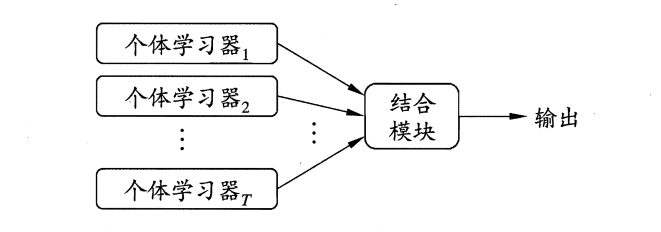
\includegraphics[width=0.8\textwidth]{../img/8-1-集成学习示意图.png}
    \caption{集成学习示意图}
    \label{fig:集成学习示意图}
\end{figure}

在集成模型中,若个体学习器都属于同一类别,例如都是决策树或神经网络,则称该集成为“同质”的(homogenneous)。同质集成中的个体学习器亦称“基学习器”(base learner),相应的学习算法称为“基学习算法”(base learning algorithm)。若个体学习器为不同类型的,则称该集成为“异质”的(heterogenous)。异质集成中的个体学习器由不同的学习算法生成,此时不再有基学习器,而称“组件学习器”(component learner)或直接称“个体学习器”。

上面我们已经提到要让集成起来的泛化性能比单个学习器好,但也存在短板效应,所以我们引入两个重要概念:准确性和多样性(diversity)。准确性指的是个体学习器不能太差,要有一定的准确度;多样性则是个体学习器之间的输出要具有差异性。

\begin{figure}[H]
    \centering
    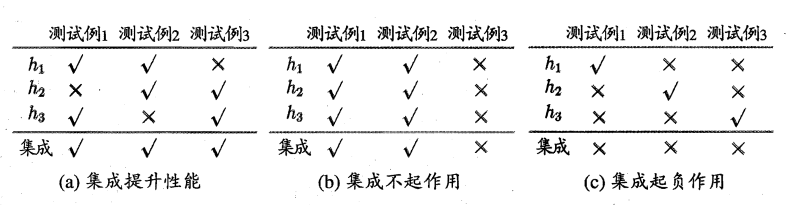
\includegraphics[width=0.8\textwidth]{../img/8-2-集成个体应“好而不同”.png}
    \caption{集成个体应“好而不同”}
    \label{fig:集成个体应“好而不同”}
\end{figure}

我们来做个简单的分析,考虑二分类问题 $y \in \{-1, +1\}$ 和真实函数 $f$,假定基分类器的错误率为 $\epsilon$,即对每个基分类器 $h_i$ 有:
\begin{equation*}
    P(h_i (x) \ne f(x)) = \epsilon
\end{equation*}

假设集成通过简单投票法结合 $T$ 个基分类器,若有超过半数的基分类器正确,则集成分类就正确:
\begin{equation*}
    H(x) = sign(\sum_{i = 1}^{T} h_i (x))
\end{equation*}

假设基分类器的错误率相互独立,则由 Hoeffding 不等式可知,集成的错误率为:
\begin{equation*}
    P(H(x) \ne f(x)) = \sum_{k = 0}^{\left \lfloor T / 2 \right \rfloor} \begin{pmatrix}
        T \\
        k
        \end{pmatrix} (1 - \epsilon)^{k} \epsilon^{T - k} \le \exp( - \frac{1}{2} T (1 - 2 \epsilon)^2)
\end{equation*}

事实上,个体学习器的“准确性”和“多样性”本身存在冲突,如何产生并结合“好而不同”的个体学习器,就是集成学习的核心。

根据个体学习器的生成方式,目前的集成学习方法大致可以分为两大类:
\begin{enumerate}[\hspace*{2em} i.]
    \item Boosting:个体学习器间存在强依赖关系、必须串行生成的序列化方法。
    \item Bagging与随机森林(Random Forest):个体学习器间不存在强依赖关系、可同时生成的并行化方法。
\end{enumerate}

\section{Boosting}

Boosting 是一族可将弱学习器提升为强学习器的算法,这族算法的工作机制类似:先从初始训练集训练出一个基学习器,再根据基学习器的表现对训练样本分布进行调整,使得先前基学习器做错的训练养你在后续受到更多关注,然后基于调整后的样本分布来训练下一个基学习器;如此重复进行,直到基学习器数目达到事先指定的值 $T$,最终将这 $T$ 个基学习器进行加权结合。

Boosting 族算法最著名的代表是 AdaBoost。AdaBoost 使用的是\textbf{指数损失函数},因此 AdaBoost 的权值与样本分布的更新都是围绕着最小化指数损失函数进行的。

定义基学习器的集成为加权结合,则有:
\begin{equation*}
    H(x) = \sum_{t = 1}^{T} \alpha_t h_t (x)
\end{equation*}
AdaBoost 算法的指数损失函数定义为:
\begin{equation*}
    loss_{\exp} (h) = \mathbb{E}_{x \sim D} [e^{- f(x) H(x)}]
\end{equation*}

具体来说,AdaBoost 算法分 3 步:
\begin{enumerate}[\hspace*{2em} i.]
    \item 初始化训练数据的权值分布,如果有 $m$ 个样本,则每个训练样本最开始时都被赋予相同的权值:$\displaystyle \frac{1}{m}$。
    \item 训练弱分类器,具体训练过程中,如果某个样本点已经被准确地分类,那么在构造下一个训练集中,它的权值就被降低;相反,如果某个样本点没有被准确分类,那么它的权值就得到提高。然后,权值更新过的样本集被用于训练下一个分类器,整个训练过程如此迭代地进行下去。
    \item 将各个训练得到的弱分类器组合成强分类器,各个弱分类器的训练过程结束后,加大分类误差率小的弱分类器的权重,使其在最终的分类函数中起着较大的决定作用,而降低分类误差率大的弱分类器的权重,使其在最终的分类函数中起着较小的决定作用。
\end{enumerate}

\begin{figure}[H]
    \centering
    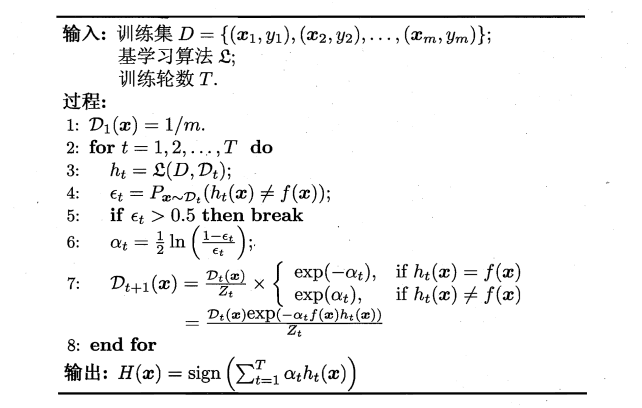
\includegraphics[width=0.8\textwidth]{../img/8-3-AdaBoost算法.png}
    \caption{AdaBoost算法}
    \label{fig:AdaBoost算法}
\end{figure}

可以看出:AdaBoost 的核心步骤就是计算基学习器权重和样本权重分布,那为何是上述的计算公式呢?这就涉及到了我们之前为什么说大部分带参机器学习算法只是改变了损失函数,就是因为大部分模型的参数都是通过最优化损失函数(可能还加个规则项)而计算(梯度下降,坐标下降等)得到,这里正是通过最优化指数损失函数从而得到这两个参数的计算公式,具体的推导过程此处不进行展开。

Boosting算法要求基学习器能对特定分布的数据进行学习,即每次都更新样本分布权重,这里书上提到了两种方法:“重赋权法”(re-weighting)和“重采样法”(re-sampling),书上的解释有些晦涩,这里进行展开一下:
\begin{enumerate}[\hspace*{2em} i.]
    \item 重赋权法:对每个样本附加一个权重,这时涉及到样本属性与标签的计算,都需要乘上一个权值。
    \item 重采样法:对于一些无法接受带权样本的基学习算法,在每一轮学习中,根据样本分布对训练集重新进行采样,再用重采样得到的样本对基学习器进行训练。大致过程为:根据各个样本的权重,对训练数据进行重采样,初始时样本权重一样,每个样本被采样到的概率一致,每次从 $m$ 个原始的训练样本中按照权重有放回采样 $m$ 个样本作为训练集,然后计算训练集错误率,然后调整权重,重复采样,集成多个基学习器。
\end{enumerate}

从偏差-方差分解来看:Boosting算法主要关注于降低偏差,每轮的迭代都关注于训练过程中预测错误的样本,将弱学习提升为强学习器。从AdaBoost的算法流程来看,标准的AdaBoost只适用于二分类问题。在此,当选为数据挖掘十大算法之一的AdaBoost介绍到这里,能够当选正是说明这个算法十分婀娜多姿,背后的数学证明和推导充分证明了这一点,限于篇幅不再继续展开。

\section{Bagging与随机森林}

上面已经提到产生“好而不同”的个体学习器是集成学习研究的核心,即在保证基学习器准确性的同时增加基学习器之间的多样性。而这两种算法的基本思(tao)想(lu)都是通过“自助采样”的方法来增加多样性。

\subsection{Bagging}

Bagging 是并行式集成学习方法,即基学习器的训练之间没有前后顺序,可以同时进行。Bagging 使用“有放回”采样的方式选取训练集,对于包含 $m$ 个样本的训练集,进行 $m$ 次有放回的随即采样操作,从而得到 $m$ 个样本的采样集,这样训练集中有接近 36.8\% 的样本没有被采到。按照相同的方式重复进行,我们就可以采集到 $T$ 个包含 $m$ 个样本的数据集,从而训练出 $T$ 个基学习器,最终对这 $T$ 个基学习器的输出进行结合。
\begin{equation*}
    \lim_{m \to \infty} (1 - \frac{1}{m})^m \to \frac{1}{e} \approx 0.368
\end{equation*}

\begin{figure}[H]
    \centering
    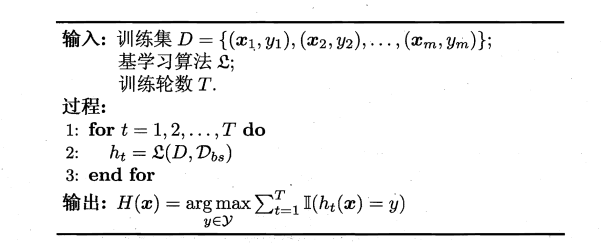
\includegraphics[width=0.8\textwidth]{../img/8-4-Bagging算法.png}
    \caption{Bagging算法}
    \label{fig:Bagging算法}
\end{figure}

可以看出Bagging主要通过样本的扰动来增加基学习器之间的多样性,因此Bagging的基学习器应为那些对训练集十分敏感的不稳定学习算法,例如:神经网络与决策树等。从偏差-方差分解来看,Bagging算法主要关注于降低方差,即通过多次重复训练提高稳定性。不同于AdaBoost的是,Bagging可以十分简单地移植到多分类、回归等问题。总的说起来则是:AdaBoost关注于降低偏差,而Bagging关注于降低方差。

\subsection{随机森林}

随机森林(Random Forest)是Bagging的一个拓展体,它的基学习器固定为决策树,多棵树也就组成了森林,而“随机”则在于选择划分属性的随机,随机森林在训练基学习器时,也采用有放回采样的方式添加样本扰动,同时它还引入了一种属性扰动,即在基决策树的训练过程中,在选择划分属性时,RF先从候选属性集中随机挑选出一个包含K个属性的子集,再从这个子集中选择最优划分属性,一般推荐 $K = \log_2 d$。

这样随机森林中基学习器的多样性不仅来自样本扰动,还来自属性扰动,从而进一步提升了基学习器之间的差异度。相比决策树的Bagging集成,随机森林的起始性能较差(由于属性扰动,基决策树的准确度有所下降),但随着基学习器数目的增多,随机森林往往会收敛到更低的泛化误差。同时不同于Bagging中决策树从所有属性集中选择最优划分属性,随机森林只在属性集的一个子集中选择划分属性,因此训练效率更高。

\begin{figure}[H]
    \centering
    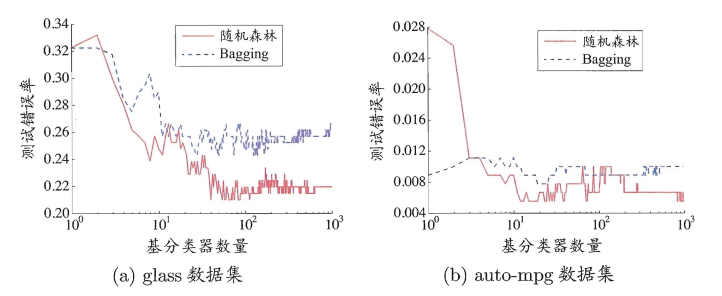
\includegraphics[width=0.8\textwidth]{../img/8-5-在两个UCI数据上,集成规模对随机森林与Bagging的影响.png}
    \caption{在两个UCI数据上,集成规模对随机森林与Bagging的影响}
    \label{fig:在两个UCI数据上,集成规模对随机森林与Bagging的影响}
\end{figure}

\section{结合策略}

结合策略指的是在训练好基学习器后,如何将这些基学习器的输出结合起来产生集成模型的最终输出。

\begin{figure}[H]
    \centering
    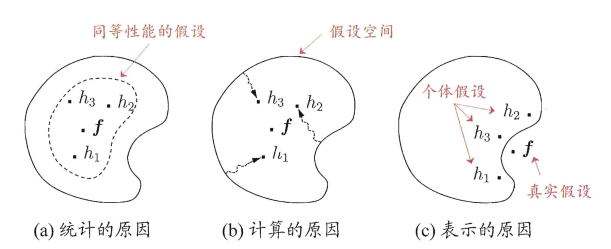
\includegraphics[width=0.8\textwidth]{../img/8-6-学习器结合可能从三个方面带来好处.png}
    \caption{学习器结合可能从三个方面带来好处}
    \label{fig:学习器结合可能从三个方面带来好处}
\end{figure}

假定集成包含 $T$ 个基学习器 $\{h_1, h_2, \cdots, h_T \}$,其中 $h_i$ 在示例 $x$ 上的输出为 $h_i (x)$。

\subsection{平均法(回归问题)}

对数值型输出 $h_i (x) \in \mathbb{R}$,最常见的结合策略是使用平均法(averaging)。

简单平均法(simple averaging):
\begin{equation*}
    H(x) = \frac{1}{T} \sum_{i = 1}^{T} h_i (x)
\end{equation*}

加权平均法(weighted averaging):
\begin{equation*}
    H(x) = \sum_{i = 1}^T w_i h_i (x)
\end{equation*}
其中 $w_i$ 是个体学习器 $h_i$ 的权重,通常要求 $w_i \ge 0, \displaystyle \sum_{i= 1}^T w_i = 1$。

易知简单平均法是加权平均法的一种特例,加权平均法可以认为是集成学习研究的基本出发点。由于各个基学习器的权值在训练中得出,一般而言,在个体学习器性能相差较大时宜使用加权平均法,在个体学习器性能相差较小时宜使用简单平均法。

\subsection{投票法(分类问题)}


\end{document}